
\documentclass{article} % For LaTeX2e
\usepackage{iclr2025_conference,times}

% Optional math commands from https://github.com/goodfeli/dlbook_notation.
\input{math_commands.tex}

\usepackage{hyperref}
\usepackage{url}
\usepackage{graphicx}


\title{Enhancing UoT with \\ Bayesian inference, multibranch, and multimodality questioning}

% Authors must not appear in the submitted version. They should be hidden
% as long as the \iclrfinalcopy macro remains commented out below.
% Non-anonymous submissions will be rejected without review.

\author{Antiquus S.~Hippocampus, Natalia Cerebro \& Amelie P. Amygdale \thanks{ Use footnote for providing further information
about author (webpage, alternative address)---\emph{not} for acknowledging
funding agencies.  Funding acknowledgements go at the end of the paper.} \\
Department of Computer Science\\
Cranberry-Lemon University\\
Pittsburgh, PA 15213, USA \\
\texttt{\{hippo,brain,jen\}@cs.cranberry-lemon.edu} \\
\And
Ji Q. Ren \& Yevgeny LeNet \\
Department of Computational Neuroscience \\
University of the Witwatersrand \\
Joburg, South Africa \\
\texttt{\{robot,net\}@wits.ac.za} \\
\AND
Coauthor \\
Affiliation \\
Address \\
\texttt{email}
}

% The \author macro works with any number of authors. There are two commands
% used to separate the names and addresses of multiple authors: \And and \AND.
%
% Using \And between authors leaves it to \LaTeX{} to determine where to break
% the lines. Using \AND forces a linebreak at that point. So, if \LaTeX{}
% puts 3 of 4 authors names on the first line, and the last on the second
% line, try using \AND instead of \And before the third author name.

\newcommand{\fix}{\marginpar{FIX}}
\newcommand{\new}{\marginpar{NEW}}

%\iclrfinalcopy % Uncomment for camera-ready version, but NOT for submission.
\begin{document}


\maketitle

\section{Introduction}

\paragraph{Motivation.}
With the growth of large language model (LLM) research, a significant amount of work has focused on improving performance on recall and knowledge-based benchmarks \cite{wang2022modernquestionansweringdatasets} as well as reasoning such as math \cite{li2024gsmpluscomprehensivebenchmarkevaluating} and multi-hop deduction \cite{zhang-etal-2024-end}. However, in many practical domains, models must be deployed in interactive environments, where they are often under-informed of the required context needed to solve a task, rendering conversational skills paramount (see Figure~\ref{fig:info_gathering_example}).

\begin{figure}[!htbp]
  \centering
  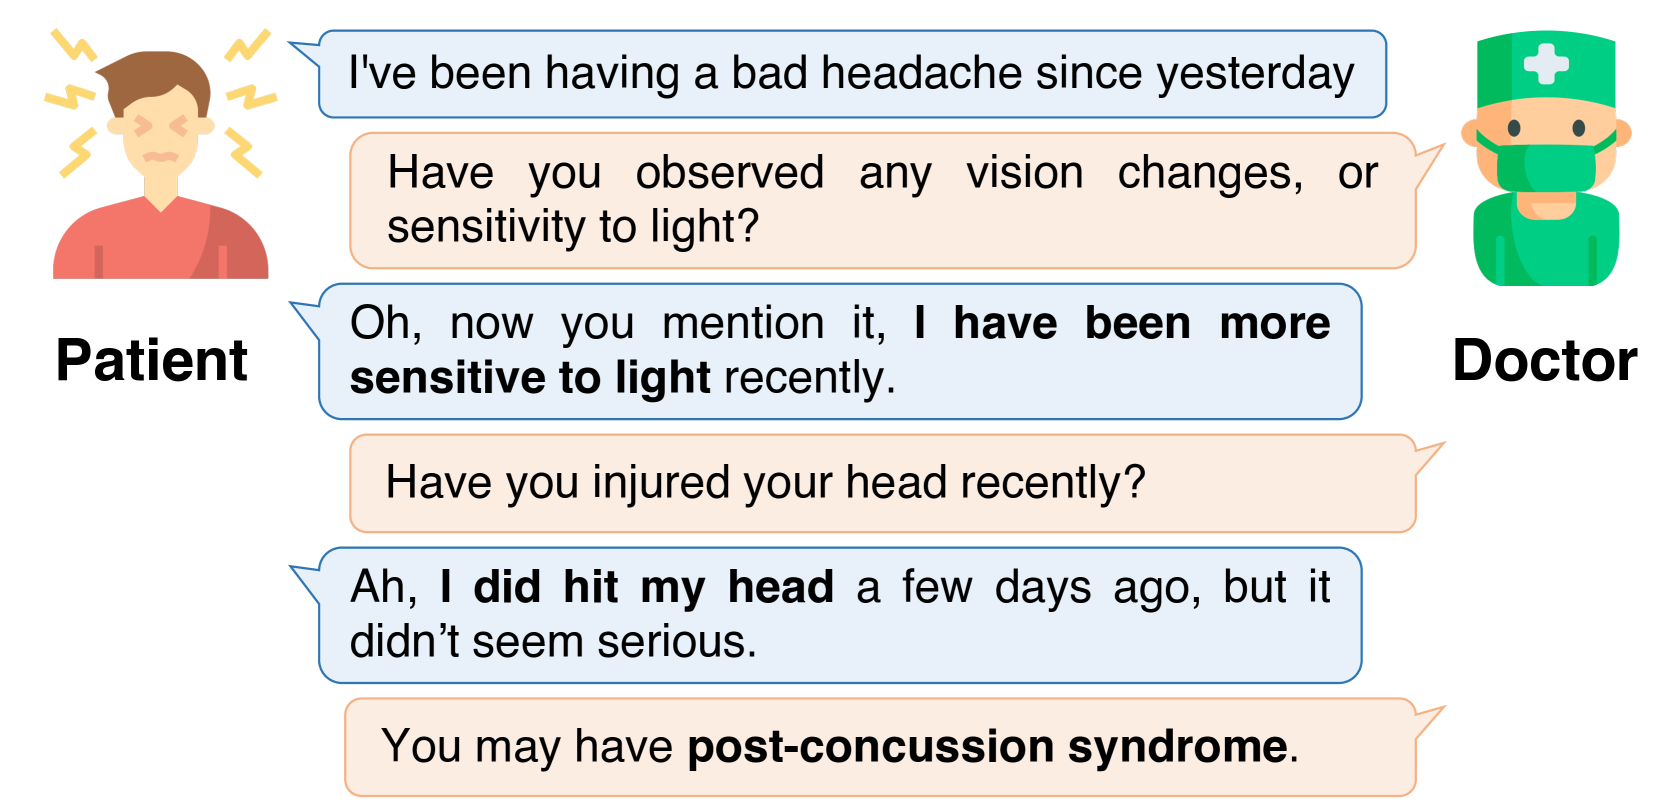
\includegraphics[width=\linewidth]{uot-example.png}
  \caption{Example from @uot on the need for conversational information acquisition in a clinical scenario}
  \label{fig:info_gathering_example}
\end{figure}

In this context, a fundamental challenge we face with current LLMs is that they depict little self-drive towards this goal \cite{goal_directedness}, and so to guide them to ask such questions effectively, we require additional techniques such as prompting \cite{wang2025learningaskllmagents}, fine-tuning \cite{alfa}, agent setups \cite{curious,ddo}, and sophisticated planning \cite{uot,mcts}.

One notable technique is \emph{Uncertainty of Thoughts (UoT)} \cite{uot}, which augments LLMs with the ability to actively request information by asking effective questions. This algorithm operates in the particular dialogical case where a model seeks to ascertain an answer from an open or closed set of possible answers. It generates binary questions (e.g., \emph{Do you have a fever?}), and simulates splitting the possible answer set into separate conversation trajectories in a tree-based graph. It then uses the simulated information gain from each trajectory to select the best question to ask its user to move the conversation forward.

Though this approach delivered a respectable performance improvement, its simplified setting brings some key limitations that remain unresolved: (1) Often we cannot discard an answer from a single question (e.g., if a patient responds \emph{No} to \emph{Do you have a fever?}, that does not discard the possibility of COVID-19) but there is still information to be gained; (2) in many conversational scenarios, it is infeasible to only ask binary questions and instead multi-branch responses are more realistic (\emph{What part of your bike is broken?} vs \emph{Are your wheels working?}, \emph{Are your handles working?}, etc.); (3) natural language responses often contain ambiguity as answerers may lack the ability to concisely and accurately reflect their thoughts.

\paragraph{Contributions.}
As a step towards resolving these limitations, we aim to extend the UoT framework with three key innovations and understand thoroughly the effect of each: (1) A Bayesian likelihood update for each possible answer rather than pruning answers; (2) multibranching to allow more than binary answers; and (3) multimodal outputs to enhance the information gain of a question. In addition, we test these against more recent interactive benchmarks such as MediQ \cite{mediq}, and provide an interactive UI for users to visualise and edit the discrimination of the search space, allowing us to provide thorough insights into the weaknesses of LLM information gathering. Our key contributions are as follows:
\begin{enumerate}
    \item We extend UoT with Bayesian probability updates for more realistic information gathering instead of harsh pruning.
    \item We extend UoT with multi-branching to allow for a wider set of more realistic questions.
    \item We extend UoT with multimodal outputs.
    \item We test these techniques on more modern interactive benchmarks including human trials, letting us more accurately assess the state of LLM information gathering.
    \item We develop an informative UI to assess the weakness areas of current LLMs at information gathering and to see how human-assisted AI can benefit.
\end{enumerate}

\section{Related Work}

\paragraph{Information Gathering.}
For humans, the importance of asking questions for reasoning \cite{Neirotti2021-xb} and cognitive development \cite{Chouinard2007-xg} is well understood to be crucial. It is no surprise then that AI/ML researchers have long explored strategies for data acquisition across multiple domains \cite{questbench}. In particular, this has become a necessary focus for LLM research for applicability to practical scenarios, where contextual knowledge is key. Retrieval-augmented generation strategies have received significant attention, with several benchmarks (\textit{citation needed}) and strategies (\textit{citation needed}) having been devised. However, despite clear evidence \cite{wu2024largelanguagemodelsask} of its importance, less attention has been brought to information acquisition in dynamic, conversational scenarios.

MediQ \cite{mediq} rigorously developed a framework for taking medical question-answer benchmarks and forming interactive patient--doctor benchmarks to test the information acquisition skills of LLMs. Against this, the authors also created a prompt-based framework where an LLM will determine whether it is confident enough to make a prediction; otherwise it will ask another question, achieving significantly better performance than direct prompting. Building on this, ALFA \cite{alfa} follows the MediQ framework on a larger dataset and proposes an alignment strategy to ask more and better questions, achieving strong results. Narrowing onto the clinical setting, authors have also found success with multi-agent models \cite{curious,ddo}, which split the task of information acquiring and diagnosis reasoning across different models. However, the above tasks have not demonstrated generalisability to other domains, nor do they consider conversation trajectories or information acquisition efficiency, limiting their applicability to real domains.

In contrast, Uncertainty of Thoughts \cite{uot} is a more generalisable framework to other domains, demonstrated on both medical and troubleshooting datasets. Though the binary split theoretically offers the most information gain, it is uncommon in practice and too aggressively prunes answers. Likewise, exploration of the whole tree is expensive. To aid in the latter, \cite{mcts} demonstrates that Monte Carlo Tree Search can be effectively applied to the UoT framework to more efficiently search the question space. % If you want strikethrough, keep the next line and load ulem.
% \sout{\cite{cip} offers an alternative model of information gain using conformal prediction sets, but it proves less effective with binary questions than UoT. \cite{handa2024bayesianpreferenceelicitationlanguage} demonstrates a very clever technique but is limited to continuous answer spaces (possibly could be extended with KNN to discrete answer sets).}
To our knowledge, though many models use acquired information for updating probable outcomes, they do not use it to judge which questions to ask in a reward system.

\paragraph{Multimodal Questions.}
A challenge for conversational LLMs is that users may struggle to specify their intent in a verbalised query. In traditional information search algorithms, multimodal information has enhanced both system and user performance (\textit{citation needed}). \cite{yuan_multimodal} extends upon this work in conversational-search algorithms aided by LLMs, discovering drastically better retrieval performance when pairing clarifying questions with relevant images.

\paragraph{Uncertainty Estimation.}
Another key requirement for LLM usage in practical scenarios is uncertainty estimation, particularly to counteract biased, hallucinated, or non-factual responses. \cite{lin2022teaching} pioneers a verbalising method where users simply ask an LLM to provide a confidence with its answer. Alternatively, one can assess the uncertainty of an answer from the latent information of a response \cite{jiang-etal-2021-know,manakul-etal-2023-selfcheckgpt,kuhn2023semantic,cole-etal-2023-selectively}, \emph{inter alia}. Where the LLM functions as a black box, \cite{cole-etal-2023-selectively} introduces sampling the consistency of responses as a means of measuring uncertainty. Comparisons between these methods generally show sophisticated latent methods perform best across multiple scenarios, though consistency lags not far behind.

Our research connects these three fields by positioning interactive information acquisition as a domain where uncertainty estimation, multimodal communication, and adaptive questioning strategies intersect. Specifically, we propose that: (1) Bayesian likelihood updates paired with uncertainty estimation enhance the nuanced understanding of information queries, and (2) multimodal questioning expands the expressive powers of interactions for more efficient information acquisition.

\section{Background}

\subsection{Probabilistic Model}
\paragraph{Hypothesis Space ($\mathcal{H}$).}
The Hypothesis Space is a discrete, mutually exclusive set of potential answers or solutions to a question, denoted by $\mathcal{H}=\{h_1,h_2,\ldots,h_n\}$. For example, in the context of a clinical diagnosis, $\mathcal{H}$ would represent the set of possible diseases.

\paragraph{Belief State ($B$).}
The Belief State is a probability distribution over the Hypothesis Space. At any step $k$, the belief state is a vector $B_k$, where the $i$-th element represents the probability of hypothesis $h_i$ given the evidence gathered so far:
\[
B_k=\big[P(h_1\mid E_{1:k}),\,P(h_2\mid E_{1:k}),\,\ldots,\,P(h_n\mid E_{1:k})\big],
\]
such that $\sum_{i=1}^{n} P(h_i\mid E_{1:k})=1$.

\paragraph{Initial Belief State ($B_0$).}
$B_0$ is the prior distribution over $\mathcal{H}$ before any evidence has been acquired. While it can be a uniform distribution (e.g., $P(h_i)=1/n$ for all $i$), a more informed prior can be based on population prevalence or domain knowledge.

\paragraph*{A preliminary method.}
Collect simple patient background (age, race, past medical history) and prompt an LLM to generate priors for illnesses, i.e., $P(h_i \mid \text{age, race, history})$. Since many priors for diseases are available online (e.g., CDC resources: \url{https://www.cdc.gov/diabetes/php/data-research/index.html}), instructing the LLM to reference sources can reduce guessing. A drawback is that not all diseases have available statistics and such priors may not generalise across tasks (e.g., in troubleshooting, background conditions are unclear across different spectra).

\subsection{Inference}
\paragraph{Evidence ($E_k$).}
At step $k$, a question $Q_k$ is posed, and the user's response constitutes the observed evidence $E_k$.

\paragraph{Likelihood Elicitation.}
For a given piece of evidence $E_k$, the system queries an LLM (prompt details to be specified) to estimate the likelihood function $P(E_k\mid h_i)$ for all $h_i\in\mathcal{H}$.

\paragraph{Uncertainty Scaling.}
To address uncertainty in LLM probability estimates, we obtain a confidence score for each likelihood, $c_i\in[0,1]$. The original likelihood is adjusted toward the neutral value $0.5$:
\[
P'(E_k\mid h_i) \;=\; c_i\,P(E_k\mid h_i) + (1-c_i)\cdot 0.5.
\]
When $c_i=1$, the adjusted likelihood equals the original; when $c_i=0$, it becomes $0.5$, which has no effect in the Bayesian update.
\textit{Note.} For simplicity, we subsequently write $P(E_k\mid h_i)$ to mean the adjusted likelihood.

% TODO: Uncertainty scaling is not final. Consider alternative strategies (e.g., Beta distributions over likelihoods; hierarchical Bayesian modelling).

\paragraph{Belief Update.}
The posterior from step $k-1$ serves as the prior for step $k$. Assuming conditional independence of evidence given a hypothesis,
\[
P(h_i \mid E_{1:k}) \;\propto\; P(h_i \mid E_{1:k-1})\, P(E_k \mid h_i).
\]
A derivation via Bayes' rule:
\begin{align*}
P(A\mid B,C)
  &= \frac{P(A,B,C)}{P(B,C)}
   = \frac{P(A,C\mid B)\,P(B)}{P(C\mid B)\,P(B)}
   = \frac{P(C\mid A,B)\,P(A\mid B)}{P(C\mid B)}.
\end{align*}
Letting $A=h_i$, $B=E_{1:k-1}$, $C=E_k$ gives
\[
P(h_i \mid E_{1:k}) \;=\; \frac{P(E_k \mid h_i, E_{1:k-1})\,P(h_i \mid E_{1:k-1})}{P(E_k \mid E_{1:k-1})}
\;\overset{\text{cond. indep.}}{=}\;
\frac{P(E_k \mid h_i)\,P(h_i \mid E_{1:k-1})}{P(E_k \mid E_{1:k-1})},
\]
with normaliser
\[
P(E_k \mid E_{1:k-1}) \;=\; \sum_{j=1}^{n} P(h_j \mid E_{1:k-1})\, P(E_k \mid h_j).
\]

\subsection{Decision Tree}
The conversational flow is modelled as a tree with two node types:
\begin{itemize}
  \item \textbf{Evidence nodes:} A state after a specific piece of evidence is received (e.g., the user answered ``Yes''). Each evidence node contains a belief state $B_k$. Its children are question nodes.
  \item \textbf{Question nodes:} A point where a question is posed. A question node has children that are evidence nodes corresponding to each possible answer.
\end{itemize}

\subsection{Optimal Question Selection}
At any evidence node, the system performs a lookahead search to determine the optimal next question, guided by an information-gain reward.

\paragraph{Shannon Entropy.}
For belief state $B$, define
\[
H(B)\;=\; -\sum_{i=1}^{n} P(h_i)\,\log_2 P(h_i).
\]

\paragraph{Information Gain.}
Let $B_{\text{parent}}$ be the belief at the parent evidence node, and $\{E_j\}$ the set of possible answers to question $Q$. With simulated evidence $E_{v:v+x}$ to depth $x$,
\begin{align*}
\operatorname{IG}(Q)
&= H(B_{\text{parent}})\;-\;\sum_{j} P\!\left(E_j \mid E_{1:k-1},E_{v:v+x}\right)\, H(B_j) \\
&= H(B_{\text{parent}})\;-\;\sum_{j}\Bigg(\sum_{i=1}^{n} P\!\left(h_i \mid E_{1:k-1},E_{v:v+x}\right)\, P\!\left(E_j \mid h_i\right)\Bigg) H(B_j),
\end{align*}
where $B_j$ is the belief after observing answer $E_j$ and $P(E_j\mid\cdot)$ its marginal. 
% TODO: Precisely specify how $P(E_j\mid\cdot)$ is computed in practice.


\paragraph{Reward formulation.}
\begin{itemize}
\item \noindent\textbf{Immediate reward $R_I$.} A scaled IG with a balance penalty controlled by $\lambda\ge 0$:
\[
R_I(Q)\;=\;\frac{\operatorname{IG}(Q)}{1+\lambda\big(\max_j P(E_j\mid E_{1:k-1},E_{v:v+x})
- \min_j P(E_j\mid E_{1:k-1},E_{v:v+x})\big)}.
\]
% TODO: UoT's reward is tailored to their task; consider alternatives.

\item \noindent \noindent\textbf{Accumulated reward $R_A$.}
From the root to the current node, defined recursively:
\[
R_A(Q)\;=\;R_I(Q)\;+\;
\begin{cases}
R_A(\mathrm{parent}(Q)), & \text{if parent}(Q)\ \text{exists},\\[2pt]
0, & \text{otherwise.}
\end{cases}
\]

\item \noindent\textbf{Expected future reward $R_E$.}
For a question $Q$ with answer branches leading to question nodes $Q'_{j,z}$,
\[
R_E(Q)\;=\;
\begin{cases}
R_A(Q), & \text{if $Q$ is a leaf of the simulation},\\[4pt]
\displaystyle \sum_{j} P(E_j)\left(\frac{1}{\rho_j}\sum_{z} R_E\!\left(Q'_{j,z}\right)\right), & \text{otherwise,}
\end{cases}
\]
where $\rho_j$ is the number of child question nodes under the evidence node for $E_j$.
% TODO: $P(E_j)$ shorthand again; specify computation route.
\end{itemize}

\subsection{The $M$-step Lookahead Algorithm}
At a given evidence node, the optimal next question is determined by lookahead simulation.

\paragraph{Hyperparameters.}
\begin{itemize}
  \item $M_q$: maximum number of candidate questions to generate at each node.
  \item $M_e$: maximum number of evidence (answer) branches per generated question.
  \item $D_{\text{sim}}$: maximum depth per iteration of the lookahead simulation.
  \item $D_{\text{ask}}$: maximum depth of the actual conversation with the user.
  \item $\tau_{\text{confidence}}$: probability threshold to consider a hypothesis confirmed.
\end{itemize}

\paragraph{Procedure.}
\begin{enumerate}
  \item \textbf{Generate:} From the current evidence node, prompt the LLM to generate up to $M_q$ question nodes with up to $M_e$ answer states.
  \item \textbf{Simulate:} For each candidate question, recursively build a simulation tree up to depth $D_{\text{sim}}$, generating further questions and updating beliefs for each potential answer.
  \item \textbf{Evaluate:} At the lowest question nodes of the simulation tree, compute $R_A$.
  \item \textbf{Backpropagate:} Compute $R_E$ for each question node, from leaves back to initial candidates.
  \item \textbf{Select:} Choose the candidate question with the highest $R_E$.
  \item \textbf{Execute \& Iterate:} Ask the selected question; transition to the evidence node matching the user’s answer; repeat.
  \item \textbf{Terminate:} Stop when some $P(h_i\mid E_{1:k}) \ge \tau_{\text{confidence}}$ or depth reaches $D_{\text{ask}}$.
\end{enumerate}

\section{Methods}

We build off UoT with three enhancements which we test in different combinations.

\paragraph{Bayesian probability updates.}
Instead of eliminating answers after a response from a question, we begin by assuming a uniform prior over the set of possible answers and instead use questions as a means of updating our priors. To ascertain the probability updates from each question, we prompt an LLM and use consistency-based uncertainty estimation to scale each response. We measure entropy directly from the probability distribution.

\paragraph{Multibranching.}
Instead of asking just ``Yes'' or ``No'' questions, we prompt the examiner LLM to give as many branches as necessary. To then match a user’s response to a particular branch, we measure the semantic similarity of both and select the maximum match.

\paragraph{Multimodal outputs.}
We also use a multimodal, RAG-equipped API LLM and prompt it to equip any question with whatever media it deems necessary.

To more thoroughly investigate where LLM information gathering fails, we also develop an interactive UI for this framework, which allows researchers to visualise the reasoning tree and modify the answer set at each node if required.

\section{Experimental Setup}

\paragraph{Datasets.}
We choose datasets that are most applicable to the answer-space reduction framework of Uncertainty of Thoughts and are representative of most downstream tasks of interest. We compare our enhancements on the same benchmarks of Uncertainty of Thoughts, including a patient-diagnosis task sampled from MedDG, a technical troubleshooting task sampled from FloDial, and the classic game, Twenty Questions, using the subset of answers selected by the original authors. We also test these enhancements on the iMedQA benchmark devised by the MediQ authors, giving us a more complete picture of how trajectory-planning approaches for information gathering compare to the alignment-based and prompting-based strategies tested on MediQ.

\paragraph{Answerer Setup.}
Conceptually, there are two actors in this framework: (1) the examiner, which generates questions and refines the answer space (e.g., the doctor); (2) the answerer, which answers questions to progress the conversation (e.g., the patient). In all cases, the examiner will be an LLM which we prompt for each necessary task. Aligned with prior research, we also use an LLM to act as the answerer given the context of its role and the conversation history. However, we also aim to conduct a human trial on one benchmark (FloDial), where people will be given a context which they ought to imagine themselves in, and use the examiner LLM to help them identify the answer. We anticipate this will show the greatest benefit in multimodal contexts, where people are more likely to struggle to verbalise their thoughts, especially without domain knowledge.

\paragraph{Models.}
Due to compute costs, we use the Deepseek-R1 API for all text-generative calls, and the Gemini~2.0 Flash API for multimodal additions. Because each answer node needs to correspond to a textual response from the answerer, we believe it is acceptable to omit the image itself from the conversation history (and simply replace it with a text summary).

\paragraph{Evaluation Metrics.}
We employ the same evaluation metrics as the Uncertainty of Thoughts paper, namely Success Rate, Mean Conversation Length, and Mean Conversation Length in Successful Cases.

\section{Ideal Results}

\begin{enumerate}
    \item Ideally the Bayesian probability updates will enhance the success rate, particularly on rarer-symptom presenting cases in the MediQ and MedDG benchmarks. If not, we can analyse the updates in probability to gain insights into where conversational deduction is failing for LLMs (e.g., is the probability and uncertainty estimation unreliable? Is epistemic uncertainty a key factor for failure? Are the questions not discriminative enough?).
    \item Ideally, the multibranching enhances the conversation efficiency, giving a reduction in mean conversation length. This makes the framework more applicable to real scenarios, where it is infeasible to ask many simple binary questions just for contextual setup. If not, the reason why would be an interesting result, because open-ended questions have already proven effective for information gathering.
    \item Ideally, multimodal questioning enhances success rate and efficiency, especially with human trials. While current research has developed LLM responders that are accurate to the context, and reasonably accurate to how a human would order the information presented, empirically, the comprehension abilities are not close to humans. For instance, the example MediQ patient dialogues demonstrate the patient having sophisticated clinical vocabulary such as ``enucleation''.
    \item Ideally, the UI will present an intuitive enough interface for the framework that we can more thoroughly understand where LLM information gathering fails. Moreover, it should permit human-aided verification and modifications, so that if the above enhancements turn out useless, we can pivot into demonstrating the effectiveness of human-aided information gathering (an unexplored area that should give good results).
\end{enumerate}

\section{Potential Limitations}

\begin{enumerate}
    \item We anticipate significant prompting challenges. Useful outputs for this scenario will involve highly structured responses, and matching outputs between the examiner and answerer may prove more difficult than expected.
    \item Compute costs. The exponential growth of the reasoning tree, especially in multi-branching, increases the number of API calls we need to make. Our rough estimate gave us $>\$350$ USD.
    \item Compute duration.
    \item The success of the paper, as it is currently framed, hinges heavily on good results, but the UI + Bayesian updates give us a good avenue to pivot into analysis/understanding of current limitations.
    \item Scope: We are still limited to the scenario where we are trying to find the correct answer from a set of possible answers. This set of possible answers must either be provided or generated by an LLM.
\end{enumerate}


\bibliography{iclr2025_conference}
\bibliographystyle{iclr2025_conference}

\end{document}
